%!TEX root = ./../thesis.tex

\chapter{Experiments}
\label{c:experiments}
In order to evaluate the current performance of the framework, a series of experiments has been conducted.
The experiments are divided into two parts, where the first part focuses on the assessment of the overall algorithm performance when executing machine learning algorithms in a distributed fashion.
For comparison Apache Spark is used as the system is currently the state-of-the-art in distributed machine learning as well as an non-parallel baseline implementation.
Besides the evaluation of the current status of the framework another motivation behind this set of experiments is to prove the usefulness of the programming model.
The second set of experiments tries to quantify how different facets of consistency management affect the algorithm performance.
Therefore the impact of communication frequency, synchronization strategy as well as various filter and merging strategies on the overall algorithm performance is evaluated.

\section{Experiment Setup}
As the algorithm for comparison, distributed lasso linear regression within the CoCoA framework is used as described in section \ref{ss:cocoa}.
Based on the generic form of convex optimization problems described in (\ref{eqn:lin_loss}), lasso linear regression is represented by
\begin{equation}
f_\alpha = \frac{1}{2} \parallel D\alpha - y \parallel^2_2
\label{eqn:lasso}
\end{equation}
and
\begin{equation}
r(\alpha) = \lambda \parallel \alpha \parallel_1
\label{eqn:lasso_reg}
\end{equation}
where $\alpha$ is the weight vector, $D$ resembles the input data together with the output $y$ and $\lambda$ is the regularization constant.
Simple randomized coordinate descent is used as the local solver within the CoCoA framework, as described in algorithm \ref{alg:scd}.
As a measure for the overall algorithm performance the distance to the optimal primal solution is used. This optimal value is calculated by running all methods for a large number of iterations (until the algorithm is converged) and then selecting the smallest primal value amongst the results.

In order to show the algorithm performance from different perspectives, two datasets with different properties such as ratio between number of examples and feature size as well as sparsity are used, as can be seen in Table \ref{tab:datasets}.
In BSP the runtime is measured on a per iteration basis on the driver for Apache Spark as well as the framework.
This includes scheduling of computation and execution.
When running stale synchronous parallel (SSP) and total asynchronous parallel (TAP) the runtime is measured for each node and iteration independently and the overall runtime is set by the best performing node.
For a better comparison between systems the data loading and setup stage is not accounted to the overall runtime.
\begin{table}[h]
\begin{center}
\begin{tabular}{ | c | c | c | c |}
\hline
\textbf{Dataset} & \textbf{Training Size} & \textbf{Feature Size} & \textbf{Sparsity} \\ \hline
epsilon & 400 K & 2 K & 1.0 \\ \hline
url & 2.4 M & 3.2 M & 3.5e-5 \\
\hline
\end{tabular}
\end{center}
\caption{Datasets for Empirical Evaluation}
\label{tab:datasets}
\end{table}

The cluster itself consists of 8 machines with each machine equipped with 16 GB of RAM and 8 Intel Xeon E3-1230 V2 CPUs running at 3.30 GHz.
All nodes are connected via 1 GBit Ethernet.
Distributed experiments running Apache Spark and the framework use 8 machines if not stated otherwise.
As a baseline, a single-core implementation of the algorithm is used.

\section{Algorithm Performance}
In order to asses the algorithm performance in comparison to Apache Spark and the baseline, lasso regression is run on the epsilon and url dataset with bulk synchronous parallel synchronization (BSP) (Section \ref{ss:synchronization}).
The algorithm hyper-parameters $\gamma$ and $\lambda$ have been tuned for best performance and are set to 1.0 and 1e-5, respectively.
\begin{figure}[ht]
\centering
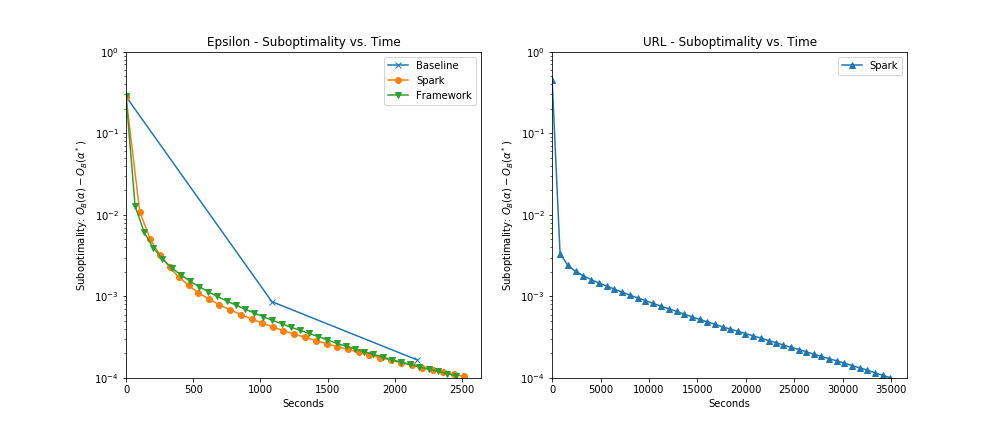
\includegraphics[width=1.0\textwidth]{img/overall_perf_cmp.png}
\caption{Overall Algorithm Performance Comparison}
\label{fig:algo_perf_cmp}
\end{figure}


\section{Consistency Management}


\subsection{Communication Frequency}
\begin{figure}[ht]
\centering
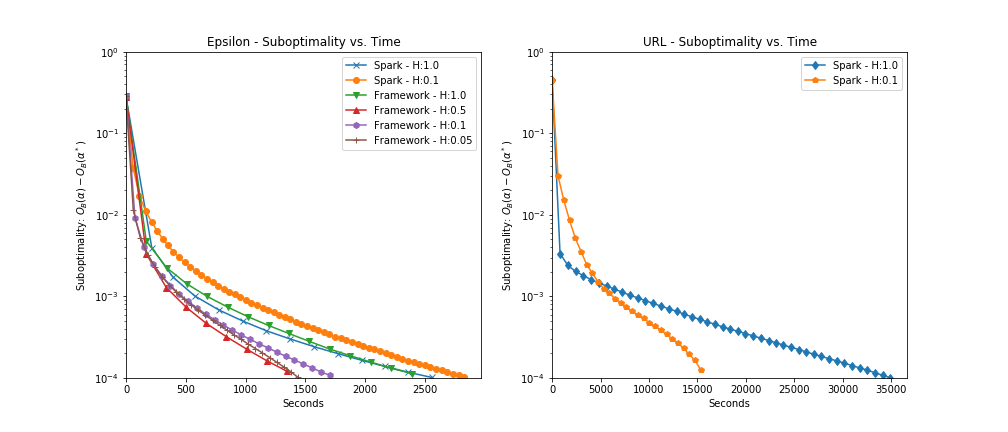
\includegraphics[width=1.0\textwidth]{img/comm_freq_cmp.png}
\caption{Communication Frequency Comparison}
\label{fig:comm_freq_cmp}
\end{figure}

\subsection{Synchronization Strategy}
\begin{figure}[ht]
\centering
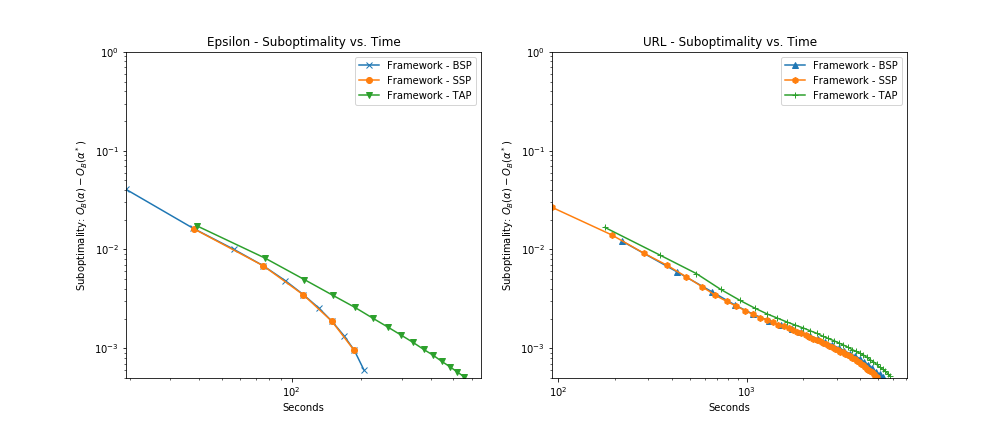
\includegraphics[width=1.0\textwidth]{img/sync_strat_cmp.png}
\caption{Synchronization Strategy Comparison}
\label{fig:sync_start_cmp}
\end{figure}

\subsection{Filtering Strategy}

\subsection{Merging Strategy}
